\chapter{Maschinelles Lernen}
\label{sec:machine_learning}
%TODO: Deutsche Begriffe, Quelle: introml

Der Bereich \glqq Maschinelles Lernen\grqq~(engl. machine learning) beschäftigt sich mit Algorithmen und Techniken zur Automatisierung von Lösungen für komplexe Probleme, die mit konventionellen Programmiermethoden schwierig umsetzbar sind. Bei der herkömmlichen Programmiermethode werden zwei verschiedene Schritte durchgeführt. Zunächst wird die Spezifikation des Programms bestimmt, um einen detaillierten Entwurf des Programms erstellen zu können. Hierbei werden Fragen, zum Beispiel \glqq Was soll das Programm können\grqq, beantwortet. Der nächste Schritt ist die Implementierung des Entwurfs mittels einer Programmiersprache\cite{IntroML}.

Die Problematik an diesem Ansatz ist, dass viele reale Probleme mit der konventionellen Methode trotz des detaillierten Entwurfs schlecht dargestellt werden können. Das Erkennen von handgeschriebenen Zeichen in einem Bild ist ein bekanntes Beispiel für diese Problematik. Der Datensatz, der aus einer großen Menge von handgeschriebenen Zeichen besteht, wird zusätzlich zu jedem Bild mit einem Label versehen, welches das handgeschriebene Zeichen wiedergibt. Letztendlich beschreibt der beschriftete Datensatz, wie sich das Programm verhalten soll. Hierbei ist das Ziel ein Programm zu entwickeln, welches die Zeichen in jedem neuen Bild erkennen soll. Dabei soll die Erkennung auch funktionieren, wenn die Bilder nicht im Datensatz vorkommen. Mit der herkömmlichen Methode wird ein allgemeiner Satz von Regeln aufgestellt, die die Beziehung zwischen den Bildern und den Zeichen beschreibt. Aufgrund der großen Unterschiede bei den handgeschriebenen Schriftzeichen kann ein solches Regelwerk eine große Herausforderung sein\cite{IntroML}.

Diese Probleme lassen sich mittels ML-Algorithmen auf einer generischen Weise lösen. Hierbei verlangen solche Algorithmen keine detaillierte Beschreibung, wie der Entwurf aussehen muss. Sie erlernen stattdessen den detaillierten Entwurf aus einem Satz von beschrifteten Daten, die das Verhalten des Programms repräsentieren. Hierbei erstellt der ML-Algorithmus ein Modell, welches er aus den beschrifteten Daten gelernt hat\cite{IntroML}.
\newpage

Da dieser Bereich in vier große Teilgebiete unterteilt werden kann, werden diese kurz vorgestellt\cite{francois}:

\begin{itemize}
	\item Unüberwachtes Lernen
	\item Überwachtes Lernen
	\item Selbstüberwachtes Lernen
	\item Bestärkendes Lernen
\end{itemize}

\section{Unüberwachtes Lernen}
%BOOK i francois

Dieser Teilbereich des maschinellen Lernens befasst sich damit, interessante Informationen aus den Eingabedaten zu ermitteln, ohne die notwendigen Labels zu benötigen. Dies kann die Visualisierung, Erfassung sowie Verarbeitung von Daten erleichtern, da sie Zusammenhänge, die in den Daten gegeben sind, besser darstellen kann. Daher ist das unüberwachtes Lernen ein notwendiger Schritt, um den Datensatz besser verstehen zu können. Dimensionalitätsreduktion und Clustering sind bekannte Anwendungen aus dem Bereich des unüberwachtes Lernens\cite{francois}.

\begin{figure}[h!]
	\centering
	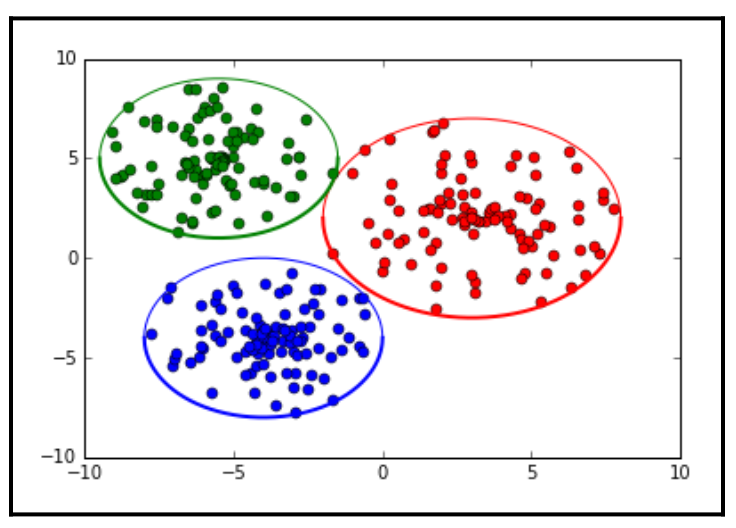
\includegraphics[width=0.7\textwidth]{bilder/cluster.PNG}
	\caption{Drei verschiedene Cluster mit den jeweiligen ähnlichen Datenpunkten werden in drei unterschiedlichen Farben visualisert\cite{Vasilev2019}.}
	\label{cluster}
\end{figure}


Beim Clustering erhält der Algorithmus eine Menge an Daten, die er in eine oder mehrere separate Gruppen (engl. Clusters) einteilt. Hierbei wird die Zuordnung der Daten anhand einer Metrik bestimmt, um die Ähnlichkeit der Daten innerhalb einer Gruppe zu maximieren sowie die Ähnlichkeit der Daten zwischen verschiedenen Gruppen zu minimieren. Dabei können Algorithmen auf verschiedene Metriken zurückgreifen, um die Ähnlichkeit messen zu können\cite{Vasilev2019}. In der Abbildung \ref{cluster} sind drei farblich unterschiedliche Gruppen zu sehen, in denen Datenpunkte ähnlich zueinander sind.




\section{Überwachtes Lernen}
%todo: deep learning erklären
Der häufigste Anwendungsfall\cite{francois} des maschinellen Lernens fällt unter dieser Kategorie. Das Ziel des überwachten Lernens (engl. supervised learning) ist das Erlernen der Zuordnung von Eingabedaten zu bekannten Ziele (engl. labels) anhand einer Menge von Beispielen. Diese Beispiele werden von Menschen erstellt. Das Lernverfahren ist daher unter menschlichem Einfluss gesteuert\cite{MLkurz}. Das erlernte System wird auf unbekannte Daten angewendet, um die Labels von bisher nicht bekannten Daten vorhersagen zu können. Die mathematische Funktion, die beim Lernverfahren gelernt werden soll, soll optimiert werden, so dass die Parameter der Funktion korrekt die bekannten Daten wiedergeben sowie unbekannte Daten vorhersehen können\cite{MLkurz}.
Fast alle Anwendungen, zum Beispiel Spracherkennung, Bildklassifizierung, Sprachübersetzung und Texterkennung, gehören zu dieser Kategorie und bestehen hauptsächlich aus Klassifizierung und Regression. Dennoch existieren einige Varianten, die nicht offensichtlich als Klassifizierung und Regression erkennbar sind. Beispiele\cite{francois} hierfür sind:

\begin{itemize}
	\item Sequenzgenerierung: Zu einem gegebenen Bild soll eine Beschriftung vorhergesagt werden, die das Bild beschreibt. Dabei kann die Sequenzgenerierung aufgrund der wiederholenden Klassifizierung eines Wortes in der Sequenz als eine Reihe von Klassifizierungsproblemen angesehen werden.
	
	\item Syntaxbaumvorhersage: Zu einem gegebenen Satz wird eine Zerlegung in einen Syntaxbaum prognostiziert.
	
	\item Objekterkennung: Bei diesem Problem wird ein minimaler Hüllkörper (engl. bounding box) um ein bestimmtes Objekt in einem gegebenen Bild gezeichnet. Als Klassifikationsproblem können die Inhalte der Hüllkörper bestimmt werden. Bei einem Regressionsproblem werden die Koordinaten des Hüllkörpers in Form eines Vektors bestimmt. 
	
	\item Bildsegmentierung: Bestimmte Objekte können mit einer pixelbasierten Maske im Bild maskiert werden.
	
\end{itemize}


\subsection{Selbstüberwachtes Lernen}

Das selbstüberwachte Lernen (engl. self-supervised learning) ist ein spezieller Fall des überwachten Lernens. Der Unterschied liegt darin, dass das Verfahren ohne von Menschen erstellten Labels arbeiten kann. Die benötigten Labels werden aus den Eingabedaten mithilfe eines heuristischen Algorithmus generiert. Bekannte Beispiele für das selbstüberwachte Lernen sind Autoencoder, dessen zu lernende und generierte Ziele die Eingabedaten sind. Autoencoder werden beispielsweise benutzt, um das nächste Einzelbild (engl. Frame) anhand von vergangenen Einzelbildern in einer Videosequenz vorherzusagen. Analog besteht die Möglichkeit, das nächste Wort in einem gegebenen Text zu prognostizieren\cite{francois}. 



\subsection{Bestärkendes Lernen}
%book f, francois, C
%theoretisch sehr viel mit quelle h

Durch das erfolgreiche Erlernen von Atari-Spielen sowie Go mittels Google DeepMind erlangte das verstärkende Lernverfahren (engl. reinforcement learning) sehr viel Aufmerksamkeit. Bei diesem Lernverfahren erhält ein Agent Informationen über seine Umgebung, um eine bestmögliche Aktion auswählen zu können. Dabei versucht er Belohnungen zu einer bestimmten Aktion zu maximieren. Zum Beispiel kann ein neuronales Netz, welches das aktuelle Einzelbild betrachtet, Spielhandlungen vorschlagen, um seine Punktzahl zu maximieren\cite{francois,Vasilev2019}. Ein solches Szenario kann mit einem verstärkenden Lernverfahren trainiert werden. Derzeit ist das Verstärkungslernen vor allem ein Forschungsgebiet und hat noch keine nennenswerten praktischen Erfolge außerhalb von Spielen erzielt. Dennoch kann dieses Verfahren im Laufe der Zeit auf Anwendungsgebiete aus der Praxis, beispielsweise selbstfahrende Autos, Robotik, Ressourcenmanagement, Bildung, ect., einen signifikanten Einfluss haben\cite{francois}.

\section{Künstliche neuronale Netze}
%BOOK 978


Die Vorbilder von künstlichen neuronalen Netzwerken sind die parallelen Strukturen von tierischen Gehirnen\cite{Bell2014}. Auf einer einfachen Form von Ein- und Ausgängen basiert grundsätzlich das Netzwerk. Aus biologischer Sicht besteht ein Neuron aus einer Zelle, welches in der Lage ist, chemische oder elektrische Signale zu verarbeiten sowie zu übertragen. Ein typisches Netzwerk setzt sich mit Neuronen zusammen, die miteinander verbunden sind. Im menschlichen Körper existieren Milliarden von Neuronen, die sich ein dichtes Netzwerk von Verknüpfungen bilden. Ein solches Neuron besteht aus drei Bestandteilen, nämlich der Eingang, welcher auch Dendrit genannt wird, der Zellkörper und der Ausgang, der als Axon bezeichnet wird. Dieser Aufbau ist in der Abbildung \ref{neural_human} veranschaulicht. 

\begin{figure}[h!]
	\centering
	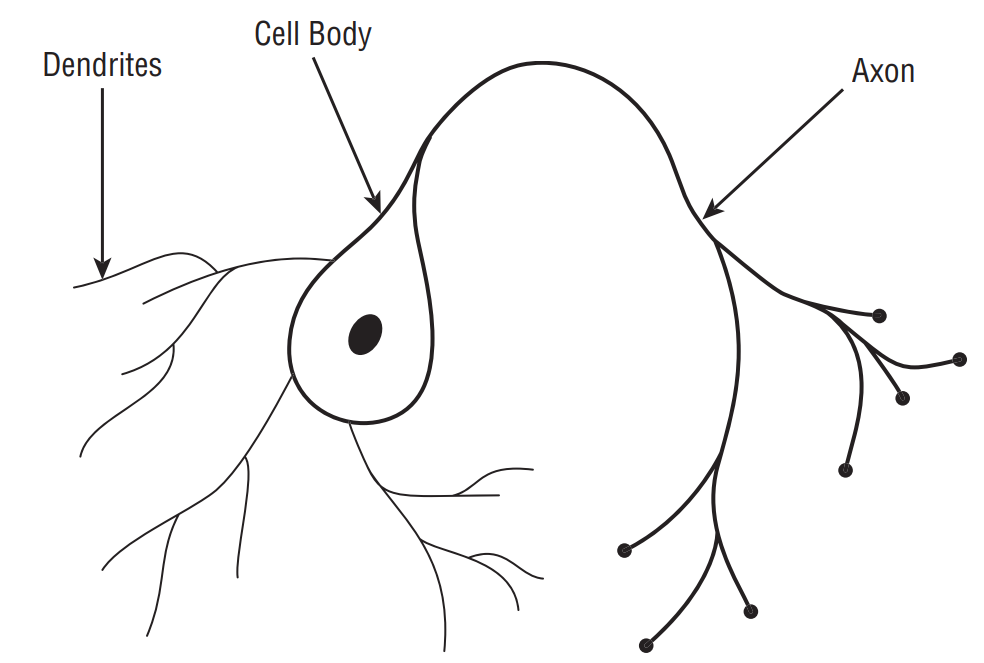
\includegraphics[width=0.7\textwidth]{bilder/neural_human.PNG}
	\caption{Vereinfachte Darstellung eines Neurons, welches aus einem Zellkörper mit den jeweiligen Ausgängen besteht\cite{Bell2014}.}
	\label{neural_human}
\end{figure}

Die Ausgänge eines Neurons werden mit den Eingängen von anderen Neuronen verknüpft, so dass ein Netzwerk aus Verknüpfungen entstehen kann. Die Komplexität von biologischen Gehirnen ist recht hoch und können bei einem Neuron 10000 verschiedene Eingänge haben. Des Weiteren werden Neuronen aktiviert, wenn das elektrochemische Signal durch das Axon gesendet wird. Das Signal erhält von dem Zellkörper eine Gewichtung. Falls ein Schwellenwert überschritten werden sollte, wird der Befeuerungsprozess durch den Ausgang entlang des Dendriten weitergeführt\cite{Bell2014}.

\subsection{Aufbau von neuronalen Netzen}
% book d Nelli2018

Die Strukturen von künstlichen neuronalen Netzen sind komplex aufgebaut. Dennoch basiert die Struktur auf einfacher grundlegender Bausteine, die innerhalb der Struktur wiederholt werden. Dadurch können komplexe Netzwerke beziehungsweise Architekturen, die von der Anzahl der grundlegenden Bausteine sowie den Typen der Verbindungen abhängig sind, entstehen, die besondere Merkmale hinsichtlich der Lernfähigkeit und der Lösung verschiedener Probleme aufweisen können. In der Abbildung \ref{network_aufbau} symbolisieren die farbigen Kreise die Basiseinheit, die auch als Knoten bezeichnet wird. Diese simulieren im biologischen Modell die Funktionalität eines Neurons in einem neuronalen Netzwerk und führen sehr einfache Operationen durch. Die Aktivierung der künstlichen Neuronen erfolgt dann, wenn die Gesamtsumme der empfangenen Eingangssignale einen bestimmten Schwellwert überschreitet. Des Weiteren können Signale zwischen den Knoten mittels Verbindungen, auch Kanten genannt, übertragen werden. Diese Verbindungen sollen die Funktionalität von biologischen Synapsen nachbilden, die in derselben Abbildung als blaue Pfeile dargestellt werden. Die Idee dahinter ist, dass das gesendete Signal von einem zu dem nächsten Neuron übertragen wird und gleichzeitig als ein Filter wirkt. Somit wandelt jede Kante, die eine Gewichtung bezüglich der Intensität hat, das Ausgangssignal eines Neurons entweder in ein hemmendes oder erregendes Signal um. Es existiert im neuronalen Netzwerk eine bestimmte Anzahl von Neuronen, die das Eingangssignal von außen annehmen können und sich in der linken Spalte in dem Netzwerkschema befinden. Diese Spalte stellt die sogenannte Eingangsschicht (engl. input layer) eines neuronalen Netzes dar (s. Abbildung \ref{network_aufbau}). In Abhängigkeit von den empfangen Eingangssignalen werden einige Neuronen aktiviert, weil das empfangene Signal verarbeitet und das Ergebnis an die andere Gruppe von Neuronen über die Kanten weitergeleitet wird. Als versteckte Schicht wird die zweite Gruppierung genannt, da sie sich zwischen dem Eingang und dem Ausgang befindet und von der nicht vorhanden Kommunikation im Eingang sowie im Ausgang mit der Außenwelt abgeschottet sind. In derselben Abbildung werden die eingehenden Kanten in der versteckten Schicht veranschaulicht, die mit allen Neuronen der vorherigen Schicht verbunden sind. Die Aktivierung der versteckten Neuronen erfolgt wie bei allen anderen Neuronen durch die Überschreitung des Schwellwerts. Nach der erfolgreichen Übertragung des Signals wird dieses verarbeitet und entweder an eine weitere Gruppe von versteckten Neuronen oder an die Ausgabeschicht (engl. output layer), die die Ergebnisse nach außen sendet, übertragen. Durch den allgemeinen Aufbau ist der Datenfluss stets von links dank der Eingabeschicht nach rechts zu der Ausgabeschicht. Letztendlich beruht die Effizienz und das Verhalten eines neuronalen Netzes auf den verbundenen Knoten, deren Verbindungen sowie die Anzahl der Schichten\cite{Nelli2018}.  


\begin{figure}[h!]
	\centering
	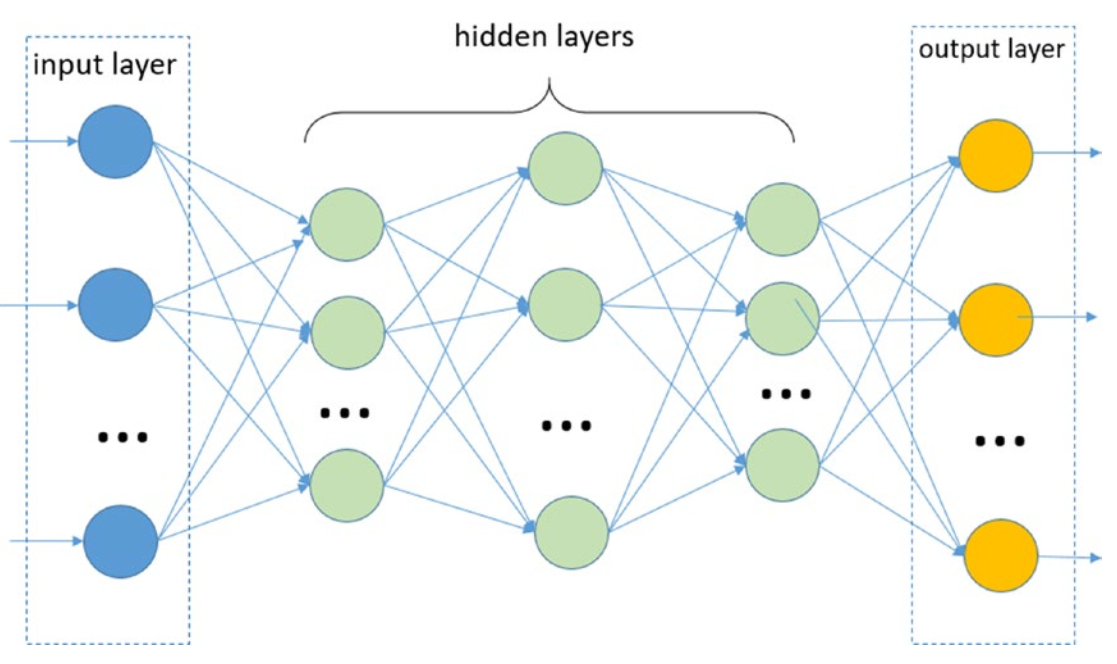
\includegraphics[width=\textwidth]{bilder/network_aufbau.PNG}
	\caption{Die Darstellung zeigt, wie ein generisches künstliches neuronales Netzwerk schematisch aufgebaut ist\cite{Nelli2018}.}
	\label{network_aufbau}
\end{figure}


\subsection{Einschichtiges Perzeptron}
%Book D \cite{Nelli2018}.

Im Jahre 1958 wurde das einfachste Modell eines neuronalen Netzes\cite{Nelli2018}, auch einschichtiges Perzeptron (engl. Single Layer Perceptron) genannt, von Frank Rosenblatt entworfen. Die Architektur ist in der Abbildung \ref{single_perz} veranschaulicht. 

\begin{figure}[h!]
	\centering
	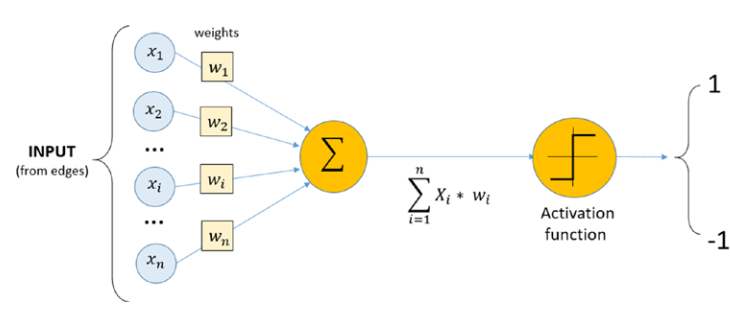
\includegraphics[width=\textwidth]{bilder/single_perz.PNG}
	\caption{Darstellung der Architektur von einem einschichtigen Perzeptron\cite{Nelli2018}.}
	\label{single_perz}
\end{figure}

\newpage
Das Modell besteht aus einer Eingabeschicht mit einer Anzahl von Neuronen, die ihre Signale mit einem Gewicht versehen und anschließend an das einzelne Neuron versenden. Die Funktionsweise des mathematischen Modells lässt sich folgendermaßen erklären. Zunächst werden die Kanten durch einen Gewichtsvektor $W$ repräsentiert:

\begin{equation}
	W = (w_1, w_2, ... , w_n)
\end{equation}

Anschließend empfängt das Ausgangsneuron ein Eingangsvektorsignal $x_i$, welches jeweils von einem anderen Neuron übermittelt wird.

\begin{equation}
X =(x_1, x_2, ... , x_n)
\end{equation}

Anschließend verarbeitet das Ausgangsneuron die Eingangssignale über eine gewichtete Summe.

\begin{equation}
	\sum_{i = 1}^{n} w_i x_i = w_1x_1 + w_2x_2 + ... + w_nx_n = s
\end{equation}

Das resultierende Signal s, welches vom Ausgangsneuron wahrgenommen wird, kann das Ausgabeneuron aktivieren, wenn es den Aktivierungsschwellenwert überschritten hat und sendet den Wert 1. Bei einer nicht erfolgreichen Aktivierung bleibt das Neuron inaktiv und verschickt den Wert -1.

\begin{equation}
\label{sp_activation}
	\text{Ausgabe} = 
	\begin{cases}
	1, & \text{wenn s$>$0}\\
	-1, & \text{sonst}
	\end{cases}
\end{equation}

Die Gleichung \ref{sp_activation} zeigt die einfachste Aktivierung. Es existieren weitere Aktivierungsfunktionen, die im Abschnitt \ref{aktivierungsfunktionen} vorgestellt werden.



\subsection{Aktivierungsfunktionen}
\label{aktivierungsfunktionen}
%TODO: Quellen!
%Book 129 \cite{Gonzalez2018}

Aus mehreren miteinander verbundenen Perzeptron-ähnlichen Einheiten besteht das neuronale Netz. Allerdings existieren Unterschiede zwischen eines neuronalen Netzes und eines Perzeptrons, wie sie das Ergebnis eines Signals verarbeiten. Die vorherige Abbildung \ref{single_perz} zeigt ein Perzeptron, welches eine Schwellenwertfunktion hat. Diese Funktion kann lediglich nur zwei Werte ausgeben, nämlich -1 und +1. Mit diesen zwei Werten führt das Perzeptron eine Klassifizierung durch. Anhand eines Beispiels lässt sich das Verhalten der Schwellenwertfunktion von einem Netzwerk aus Perzeptronen illustrieren. Angenommen, in diesem Netzwerk ist die Ausgabe vor dem Schwellenwert einer der Perzeptronen winzig klein und größer als null. Wenn der Schwellenwert erreicht wird, wird dieses sehr kleine Signal in ein +1 umgewandelt. Dennoch kann ein ähnlich kleines Signal mit dem entgegengesetzten Vorzeichen zu großem Wertumschwung von +1 nach -1 führen. Da neuronale Netze aus Schichten von Knoteneinheiten gebildet werden, bei denen die Ausgabe eines Knotens das Verhalten aller ihr folgenden Knoten beeinflussen kann, führt diese Empfindlichkeit gegenüber kleiner Signale zu Stabilitätsproblemen. Deswegen sind Perzeptronen für diese Architektur ungeeignet. Diese Problematik lässt sich lösen, in dem die Aktivierungsfunktion von einem hart beschränkten auf eine glatte, sanfte Funktion verändert wird\cite{Gonzalez2018}. Die bekannteste Aktivierungsfunktion ist die sogenannte Sigmoid-Funktion:

\begin{equation}
\label{sigmoid}
	h(z) = \frac{1}{1 + \exp(-z)}
\end{equation}

Die Variable $z$ entspricht der Summe eines berechneten Neurons. Der Vorteil an solchen glatten Funktionen liegt darin, dass sie leicht ableitbar sind.

\begin{equation}
\label{ableitung_sig}
	h'(z) = \frac{\partial h(z)}{\partial z} = h(z)[1 - h(z)]
\end{equation}


Die Abbildung \ref{aktivierung} zeigt drei verschiedene Aktivierungsfunktionen, die sehr häufig im Kontext des neuronalen Netzes verwendet werden. Der linke Graph entspricht der von der Gleichung \ref{sigmoid} bekannten Sigmoid-Funktion. Diese hat eine gestauchte S-Form und die Funktionswerte befinden sich zwischen 0 und 1. Im Vergleich zu der hyperbolischen Tangensfunktion hat diese Funktion keine starke Stauchung der S-Form. Des Weiteren sind die Funktionswerte im Bereich zwischen 1 und -1. Die rechte Funktion ist die ReLU-Funktion (Rectifier linear unit). Diese zeichnet sich aus, negative Eingabewerte auf den Wert null zu normieren. Des Weiteren neigt diese Funktion dazu, bessere Leistungen bei tiefen neuronalen Netze zu zeigen\cite{Gonzalez2018}.

\begin{figure}[h!]
	\centering
	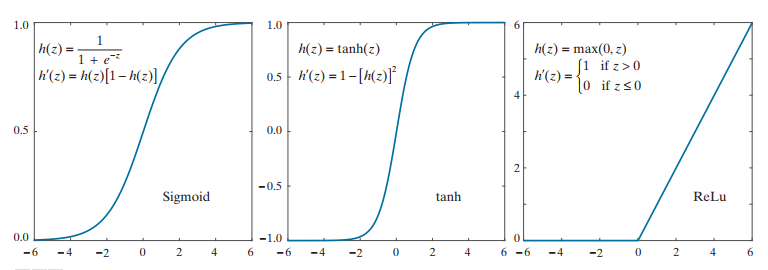
\includegraphics[width=\textwidth]{bilder/aktivierung.PNG}
	\caption{Hier sind drei Aktivierungsfunktionen zu sehen. Die linke Abbildung veranschaulicht die Sigmoid-Funktion. Anschließend folgt die hyperbolische Tangensfunktion. Die letzte Abbildung ist die sogenannte ReLU-Funktion \cite{Gonzalez2018}.}
	\label{aktivierung}
\end{figure}

\newpage
Weiterhin existieren weitere Aktivierungsfunktionen, die hier kurz beschrieben werden\cite{Vasilev2019}:

%book h
\begin{itemize}
	\item Identitätsfunktion: $f(a) = a$ \newline Diese Funktion bewirkt, dass der Aktivierungswert unverändert durchlaufen wird. 
	
	\item Schwellenwertaktivitätsfunktion: f(a) = 
	$\begin{cases}
		1, & \text{wenn a$\geq$0}\\
		0, & \text{wenn a$<$0}
	\end{cases}$
	\newline Wenn die Aktivierung über einem bestimmten Wert liegt, dann aktiviert diese Funktion das Neuron.
	
	\item bipolare Sigmoid-Funktion: $f(a) = \frac{1-\exp(-a)}{1+\exp(-a)}$ \newline Diese Funktion entspricht der stochastischen Sigmoid-Funktion, die neu skaliert und verschoben wurde, um den Wertebereich zwischen -1 und 1 zu erhalten.
	
\end{itemize}


\subsection{Lernverfahren}

Da die Gewichte der Kanten noch unpassend sind, müssen neuronale Netze dementsprechend diese lernen. Auf iterative Weise lernt das neuronale Netz. Hierbei wird eine Anzahl von Zyklen durchgeführt, um die Gewichte der Kante leicht verändert anpassen zu können. Jeder Lernzyklus entspricht einer Epoche. Für das Lernverfahren werden Eingabedaten, auch Trainingsdaten genannt, benötigt. Für jeden Eingangswert wird der erwartete Ausgangswert ermittelt, um einen Vergleich mit dem Ausgabewert, welcher von dem neuronalen Netz stammt, durchzuführen. Die Differenz zwischen den Eingabewerten sowie den erzeugten Ausgabewerten ist die Grundlage für die Veränderung der Gewichtswerte. Mithilfe einer Kostenfunktion, die das Ziel einer Minimierung hat, werden die Gewichte der verschiedenen Kanten für jede Epoche angepasst. Nach Abschluss der Lernphase folgt die Evaluierungsphase. In dieser Phase wird das trainierte neuronale Netz einen anderen Satz von Eingabewerten, hier Testdatensatz, verwenden, um die Ergebnisse evaluieren zu können. Durch die Bewertung der Differenzen zwischen den erhaltenen und den erwarteten Werten wird der Fähigkeitsgrad des neuronalen Netzes ermittelt. Der Prozentsatz der Fälle, der mit den falschen Werten prognostiziert wurde, wird verwendet, um die Genauigkeit (engl. accuracy) zu beziffern \cite{Gonzalez2018,IntroML,Vasilev2019}.


\subsubsection{Gradientenabstieg}

Dieser Abschnitt basiert auf dem Buch von Gopinath Rebala, Ajay Ravi und Sanjay Churiwal\cite{IntroML}.
\newline
Der voraussagte Wert $y_p$ hat eine bestimmte Form, die bei dem Gradientenabstieg ausgenutzt wird. Diese Form lässt sich folgendermaßen beschreiben:

\begin{equation}
y_p = h_0 = \theta_0 * x_0 + \theta_1 * x_1 + ... + \theta_n * x_n
\end{equation}

Der Fehler aus dem gegebenen Datensatz lässt sich mit der Differenz zwischen dem vorausgesagten und beobachteten Wert, also $y_p-y$, ermitteln. Der Gesamtfehler über $m$ Datenpunkte ist durch diese Gleichung gegeben:

\begin{equation}
\label{quad_fehler}
J(\theta) = \frac{1}{2m}\sum_{i=1}^{m}(h(x^i) - y^i)^2
\end{equation}

Der Termausdruck $h(x^i)$ stellt den vorhergesagten Wert $y_p$ für den i-ten Datenpunkt dar. Anschließend wird der gesamte Ausdruck in der Summe quadriert, um jeden Fehler positiv darzustellen und somit die gegenseitige Aufhebung der Summe zu vermeiden. Um den Durchschnitt der Summe zu erhalten, wird die Summe durch den Wert $2m$ dividiert. Typischerweise sind Kostenfunktionen, beispielsweise Gleichung \ref{quad_fehler}, quadratisch, so dass die Form der Funktion parabelförmig ist. Die Abbildung \ref{parabel} zeigt diese typische Form, die gewisse Eigenschaften hat.


\begin{figure}[h!]
	\centering
	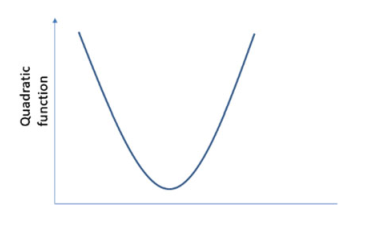
\includegraphics[width=0.55\textwidth]{bilder/quadratic_func.PNG}
	\caption{Visualisierung der allgemeinen Form einer quadratischen Gleichung. Diese entspricht einer Parabel\cite{IntroML}.}
	\label{parabel}
\end{figure}

\newpage
Zunächst hat die Abbildung genau einen Minimum-Wert. Des Weiteren existiert ein lokales Minimum, so dass alle Werte, die außerhalb des Minimums liegen, größer sind. Außerdem sagt das Vorzeichen der Steigung aus, ob der Gradient links oder rechts von dem Minimum liegt. Der Gradient wird auf dieser Kurve zum Minimum hin absteigen, wobei die Steigungsrichtung und der Wert als Orientierungshilfe verwendet werden. Letztendlich nutzt der Gradientenabstieg für die Lösung des Verfahrens genau diese drei genannten Eigenschaften. 





\paragraph{Bestimmung der Steigung}
%%book c

~\newline

Von den Koeffizienten $\theta_0$ bis $\theta_n$ hängt die Kostenfunktion $J(\theta)$ ab. Diese Koeffizienten müssen bestimmt werden. Dieses Verfahren, das das Finden von Gradienten in Bezug auf nur eine Variable realisiert, wird auch als partielle Ableitung bezeichnet und mit dem Symbol $\partial$ gekennzeichnet. Zum Beispiel stellt $\frac{\partial J}{\partial \theta_0}$ die Steigung von $J(\theta)$ in Bezug auf $\theta$ dar.
Die Ableitung von der Kostenfunktion (s. Gleichung \ref{quad_fehler}) hat eine einheitliche Darstellung in allen $\theta_j$ ($j = (0,1,2...,n)$:

\begin{equation}
\label{ableitung_partial}
\frac{\partial J}{\partial \theta_j} = \frac{1}{m}\sum_{i=1}^{m}(h(x^i) - y^i)*x_j^i
\end{equation}

\paragraph{Anpassung/Korrektur}
~\newline



Nach der Initialisierung der $\theta$-Koeffizienten mit zufälligen Zahlen kann die Steigung von der Kostenfunktion $J(\theta)$ bezüglich $\theta_j$ bestimmt werden. Anschließend werden alle Koeffizienten mit dem berechneten Wert aktualisiert:

\begin{equation}
\label{}
\theta_j = \theta_j - \alpha*\frac{\delta J}{\delta\theta_j}
\end{equation}

Dabei entspricht $\alpha$ einer Konstante und dient als Korrekturfaktor. Wenn die berechnete Steigung positiv ist, dann wird der Term $\theta_j$ kleiner. Analog gilt es auch für die negative Steigung, die den Wert $\theta_j$ größer macht. Dies wird solange wiederholt, bis das Minimum der Kostenkurve erreicht wurde. 


\paragraph{Lernrate}
~\newline


Da die Gleichung \ref{ableitung_partial} nur die Steigung berechnet und nur die Richtung angibt, ob $\theta_j$ erhöht oder erniedrigt werden soll, wird ein Mechanismus benötigt, welches der Aktualisierung mitteilt, wie weit in eine bestimmte Richtung aktualisiert werden darf. Ein solcher Mechanismus $\alpha$ wird auch als Lernrate bezeichnet.

\begin{figure}[h!]
	\centering
	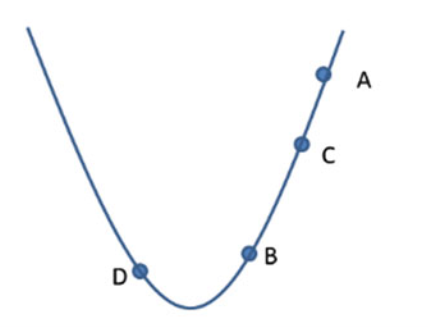
\includegraphics[width=0.65\textwidth]{bilder/quadratic_func_labeled.png}
	\caption{Visualisierung der Kostenfunktion mit vier verschiedenen Punkten, die durch eine bestimme Lernrate erreicht werden kann.\cite{IntroML}.}
	\label{lernrate}
\end{figure}


Die Abbildung \ref{lernrate} zeigt eine Kostenfunktion mit vier verschiedenen Punkten. Ausgehend von der Position A wird die Steigung berechnet. Um das Minimum zu erreichen, muss der Wert $\theta_j$ in die linke Richtung aktualisiert werden. Diese Information ist in der Steigung aufgrund des positiven Wertes gegeben. Eine hohe Lernrate sorgt dafür, dass ein großer Schritt in Richtung des Minimums gemacht wird, so dass der Punkt B erreicht wird. Allerdings kann es bei der nächsten Iteration sein, dass das Minimum übersprungen wurde und $\theta_j$ sich bei dem Punkt D aufhält. Bei einer kleinen Lernrate wird beispielsweise der Punkt C ausgehend von Punkt A erreicht. Die Konsequenz aus einer kleinen Lernrate ist, dass viel öfter iteriert werden muss, um das Minimum zu erreichen. Außerdem dauert die Berechnung dadurch länger. Die Berechnungen werden solange fortgeführt, bis die Lösung des gewünschten Wertes konvergiert.

%%abschnitt konvergenz erstmal rausgelassen

\subsubsection{Fehlerrückführung}


%978

Die Fehlerrückführung (engl. back propagation) berechnet die Gradienten und ordnet dementsprechend die richtigen Eingänge den richtigen Ausgängen zu. Das Verfahren besteht aus zwei Schritten, nämlich die Propagationsphase sowie die Aktualisierung der Gewichte aller Neuronen. Der Pseudocode \ref{pseudo_back} fasst die notwendige Schritte zusammen. Zunächst werden die Gewichte mit zufälligen Werten in der Propagationsphase bereitgestellt. Anschließend werden die Beispiele aus dem Datensatz mit dem Modell klassifiziert und deren Fehler bestimmt. In der Fehlerrückführungsphase werden die Gewichte jeweils von der versteckten Schicht zur Ausgabeschicht sowie von der Eingabeschicht zur versteckten Schicht berechnet, um die aktuelle Gewichte des Netzwerks aktualisieren zu können\cite{Bell2014}.

\begin{lstlisting}[caption={Der Pseudocode zu dem Fehlerrückführung-Algorihtmus beschreibt die notwendigen Schritte\cite{Bell2014}.}, label=pseudo_back]
Initialisierung der Gewichte mit Zufallswerten;
while(Beispiele noch vorhanden):
	Für jedes Beispiel x:
		Vorhersage  = neural_output(network, x)
		aktuell  = korrektes_label(x)
		Fehler ist (Vorhersage - aktuell) an den Ausgabenknoten;
		
Fehlerrückführung:
	- Berechne Gewichte von der versteckten Schicht zur Ausgabeschicht;
	- Berechne Gewichte von der Eingabeschicht zur versteckten Schicht;
	- Aktualisiere Gewichte von dem Netzwerk bis alle korrekt anhand der Trainingsdaten klassifiziert wurden;
	- Rückgabe des abgeschlossenen Netzwerks;
\end{lstlisting}



% book h backpropagation seite 55

%%%%%%%%%%%%%%%%%%%%%%%%%%%%%%%%%%%%%%%%%%%%%%%%%%%%%%%%%%%%%%%%%%%%%%%%%%%%%%%%%%%%%%
% 129 seite 953
%TODO: Zeilenumbrüche, ell und L unterschied

\paragraph{Mathematischer Hintergrund}
~\newline

In diesem Abschnitt wird der Pseudocode aus der Perspektive der Mathematik betrach-\newline tet\cite{Gonzalez2018}.
\newline

Um die Parameter des neuronalen Netzes finden zu können, werden die Trainingsdaten benötigt, um den Fehler zu minimieren. Mittels einer Fehlerfunktion wird der Durchschnitt der Unterschiede zwischen gewünschten und tatsächlichen Antworten gemessen. Die Variable \textbf{r} soll die gewünschte Antwort für einen gegebenen Mustervektor \textbf{x} repräsentieren. Des Weiteren beschreibt \textbf{a}(\texttt{L}) die tatsächliche Antwort des Netzes zu der Eingabe. 


Die Aktivierungswerte von dem Neuron \texttt{j} in der Ausgabeschicht werden als $a_j$(\texttt{L}) bezeichnet. Der Fehler dieses Neurons wird folgendermaßen für $j = 1,2,...,n\texttt(L)$ definiert:

\begin{equation}
\label{fehler_E}
	E_j = \frac{1}{2}(r_j - a_j(L))^2
\end{equation}

Für ein gegebenes Muster $x$ ist $r_j$ die gewünschte Antwort des Ausgangsneurons $a_j$(\texttt{L}). Der Ausgabefehler zu einem einzelnen Muster ist die Summe der Fehler aller Ausgabeneuronen:

\begin{equation}
E = \sum_{j = 1}^{n_L}(r_j -a_j(L))^2 \\\\
 = \frac{1}{2}\Vert{r - a(L)}\Vert^2
\end{equation}

Diese Summe lässt sich auch als euklidische Vektornorm definieren. Der Gesamtfehler aller Trainingsmuster ist als die Summe der Fehler der einzelnen Muster definiert. Das Ziel ist hierbei Gewichte mithilfe des Gradientenabstiegs zu finden, welche diesen Gesamtfehler minimieren. Da wir die Gradienten der Gewichte in den versteckten Knoten nicht berechnen können, wird der Backpropagation-Algorithmus verwendet, welcher den Ausgabefehler in das Netzwerk weiterleiten kann. Um dies zu ermöglichen, muss die Frage beantwortet werden, wie sich der Fehler \texttt{E} bezüglich der Gewichte im Netzwerk ändert. Der Ausdruck $\partial E/\partial z_j(\ell)$ ist die Steuergröße für die Anpassung, wobei $\partial z_j(\ell)$ die Netzeingabe zu dem Knoten $j$ in der $\ell$-Schicht ist. Zur Vereinfachung wird ein neues Symbol $\delta_j(\ell)$ eingeführt, das den Ausdruck $\partial E/\partial \delta_j(\ell)$ repräsentiert. Der Backpropagation-Algorithmus beginnt zunächst mit der Ausgabe: 

\begin{equation}
\label{delta_hidden}
\delta_j(L) = \frac{\partial E}{\partial z_j(L)}
\end{equation}

%\begin{equation}
%12.54 nötig??
%\end{equation}

Mithilfe der Kettenregel kann dieser Ausdruck in Bezug auf die Ausgabe $a_j(L)$ weiter umformuliert werden:

\begin{equation}
\delta_j(L) = \frac{\partial E}{\partial z_j(L)} = \frac{\partial E}{\partial a_j(L)}\frac{\partial a_j(L)}{\partial z_j(L)} = \frac{\partial E}{\partial a_j(L)}\frac{\partial h(z_j(L))}{\partial z_j(L)}
\newline =  \frac{\partial E}{\partial a_j(L)}h'(z_j(L))
\end{equation}

Das Symbol $h$ soll die Aktivierungsfunktion darstellen, die die Netzeingabe $z_j$ in der letzten Schicht $L$ als Parameter hat. Die Ableitung der Aktivierungsfunktion ist aus der Gleichung \ref{ableitung_sig} bekannt. Des Weiteren lässt sich der Fehler (s. Gleichung \ref{fehler_E}) nach $a$ ableiten. Die Gleichung sieht nun folgendermaßen aus:  

\begin{equation}
\delta_j(L) = h(z_j(L))[1 - h(z_j(L))] [a_j(L) - r_j]
\end{equation}

Der Termausdruck $h(z_j(L))]$ ist bekannt, wenn durch alle Neuronen von der ersten bis zu der letzten Schicht im Netzwerk traversiert wurde. Die Aktivierungswerte $a_j(L)$ können in der Ausgabe des Netzwerks beobachtet werden. Außerdem ist die Variable $r_j$ mit dem Muster $x$ während des Trainings ersichtlich und somit kann der Ausdruck $\delta_j(L)$ berechnet werden. 
Da die Beziehung zwischen dem Netzeingang und dem Ausgang eines beliebigen Neurons in einer beliebigen Schicht $\ell$ gleich ist, gilt die Gleichung \ref{delta_hidden} für jeden Knoten $j$ in einer versteckten Schicht:

\begin{equation}
\label{zujedemneuron}
\delta_j(\ell) = \frac{\partial E}{\partial z_j(\ell)}
\end{equation}

Die Gleichung \ref{zujedemneuron} beschreibt, wie sich der Fehler in Bezug auf eine Änderung des Netzeinganges zu jedem Neuron im Netzwerk ändert. Der nächste Schritt ist den Ausdruck $\delta_j(\ell)$ in Form von $\delta_j(\ell + 1)$, umzuformulieren. Da der Fehler im Netzwerk rückwärts zurückgeführt werden soll, ist die Beziehung zwischen den beiden Ausdrücken unabdingbar, um den Ausdruck $\delta_j(L - 1)$ ausgehend von $\delta_j(L)$ zu finden. Das gefundene Ergebnis wird weiter verwendet, bis die zweite Schicht und so weiter erreicht wurde. Mithilfe der Kettenregel kann der gewünschte Ausdruck formuliert werden:

\begin{equation}
\begin{split}
	\delta_j(\ell) = \frac{\partial E}{\partial z_j(\ell)} = \sum_{i}\frac{\partial E}{\partial z_j(\ell + 1)} \frac{\partial z_j(\ell + 1)}{\partial a_j(\ell)}\frac{\partial a_j(\ell)}{\partial z_j(\ell)}  \\
	= \sum_{i}\delta_i(\ell + 1) \frac{\partial z_j(\ell + 1)}{a_j(\ell)}h'(z_j(\ell)) = h'(z_j(\ell))\sum_{i}\omega_{ij}(\ell + 1)\delta_i(\ell + 1)
\end{split}
\end{equation}

In der Gleichung gilt $\ell = L-1, L-2,...,2$. Die aktuelle Antwort des Netzwerks $a_j$ kann durch $h'(z_j(\ell))$ ersetzt werden. Des Weiteren wird die Gleichung \ref{zujedemneuron} angewendet, um zu der letzten Formulierung zu gelangen. Die Gesamteingangsgröße $z_i$ für das Neuron $i$ in der Schicht $\ell$ lässt sich auch als Summe der Gewichte von jeweiligen Kanten mit den Antworten der vorherigen Schicht beschreiben.
Der aktuelle Stand ist, dass der Fehler bei der Ausgabe berechnet werden kann. Des Weiteren steht eine Funktion zur Verfügung, die die Veränderung des Fehlers zu jedem Knoten im Netzwerk beschreiben kann. Der nächste Schritt ist nun, den Ausdruck $\partial E/\partial w_{ij}$ in Bezug auf $\delta_j(\ell)=\partial E/z_j(\ell)$ zu erhalten. Auch hierfür wird die Kettenregel nochmal angewendet:

\begin{equation}
\frac{\partial E}{\partial \omega_{ij}(\ell)} = \frac{\partial E}{\partial z_i(\ell)}\frac{\partial z_i(\ell)}{\partial \omega_{ij}(\ell)} = \delta_i(\ell)\frac{\partial z_i(\ell)}{\partial \omega_{ij}(\ell)} = a_j(\ell - 1)\delta_i(\ell)
\end{equation}

Die Gleichung \ref{zujedemneuron} wurde verwendet, um die Umformung zu vereinfachen. Außerdem entspricht der Ausdruck $\partial z_i(\ell)/\partial \omega_{ij}(\ell)$ dem Term $a_j(\ell - 1)$. 
Da die Änderungsrate von $E$ in Bezug auf die Gewichte berechnet werden kann, ist nun die Aktualisierung der letzte Schritt:


% bias raus erstmal
%\begin{equation}
%\frac{\partial E}{\partial b_i(\ell)} = \delta_i(\ell)
%\end{equation}


\begin{equation}
\omega_{ij}(\ell) = \omega_{ij}(\ell) - \alpha\frac{\partial E(\ell)}{\partial \omega_{ij}(\ell)} = \omega_{ij}(\ell) - \alpha\delta_i(\ell)a_j(\ell - 1)
\end{equation}

Die Lernrate $\alpha$ wird bei dem Vorwärtspass berechnet und bei dem Gradientenabstieg verwendet. Die Berechnungen von $\delta$ werden während des Backpropagation-Algorithmus ermittelt. 



%%bias ignorieren
%\begin{equation}
%b_i(\ell) = b_i(\ell) - \alpha \frac{\partial E}{\partial b_i(\ell)} = b_i(\ell) - \alpha \delta_i(\ell)
%\end{equation}


\section{Convolutional Neural Networks}
%Begriffe poolingschicht ect einheitlich

Die mathematische Faltung ist ein sehr wichtiges Konzept aus dem Bereich des maschinellen Lernens. Mithilfe der Faltung können wichtige Merkmale automatisiert extrahiert werden, die zur Identifizierung der Zielklassen benötigt werden\cite{IntroML}. Der Vorteil liegt darin, dass dieser Ansatz alle räumlichen Beziehungen nutzt, die zwischen Pixeln in einem Bild bestehen können, zum Beispiel Pixelanordnungen in Ecken, das Vorhandensein von Kantensegmenten und anderen Merkmalen, um ein Bild von einem anderen unterscheiden zu können. Daher wird in diesem Abschnitt eine neue Klasse von neuronalen Netzwerken vorgestellt, die als Convolutional Neural Networks (engl. CNN) bezeichnet werden. Außerdem können solche Netze Bilder als Eingabe akzeptieren und eignen sich für das automatische Lernen und die Bildklassifizierung\cite{Gonzalez2018}.

\subsection{Aufbau}

Der allgemeine Aufbau von Faltungsnetzen\cite{Gonzalez2018, IntroML} besteht aus mehreren Schichten von Faltungsschichten zu Poolingschichten, die oft wiederholt werden, um lokale Merkmale aus Eingangsbildern zu lokalisieren und anschließend diese mathematisch zu falten sowie die Dimension des Bildes zu reduzieren. Durch diese Vorgehensweise können Merkmale gefunden werden, die in sehr abstrakter Form vorliegen. Nach einer bestimmten Anzahl von Wiederholungen der Schichten folgt ein klassisches neuronales Netz, welches die Klassifikation durchführt. Die generelle Funktionsweise von Faltungsschichten und Poolingschichten werden in den Abschnitten \ref{sec:faltungsschicht} und \ref{sec:poolingschicht} erläutert. 

Die Abbildung \ref{cnn_arch} visualisiert den klassischen Aufbau eines Faltungsnetzes. Das Faltungsnetz nimmt ein Bild als Eingabe an. Mithilfe der Faltungsschicht wird die Eingabe abgetastet und mathematisch gefaltet. Dadurch entstehen mehrere Feature-Maps, dessen Dimensionen in anschließendem Schritt reduziert wird. Dann folgt wieder eine Faltungsschicht, die die Anzahl der Feature-Maps erhöht. Daraufhin wird ein letztes Mal eine Poolingschicht angewendet. Anschließend kann ein klassisches neuronales Netz Feature-Maps als Vektor annehmen, um eine Klassifikation durchführen zu können\cite{Gonzalez2018}.

\begin{figure}[h!]
	\centering
	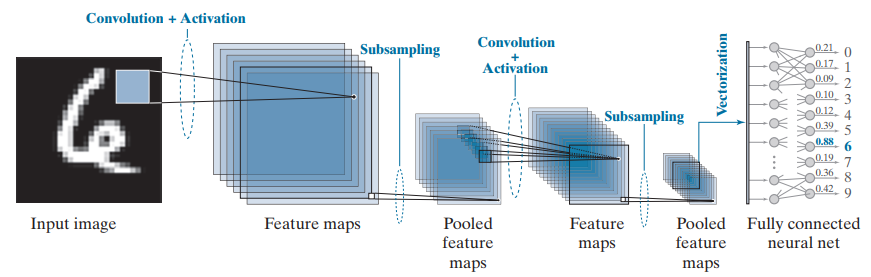
\includegraphics[width=\textwidth]{bilder/cnn_arch.PNG}
	\caption{Darstellung der verschiedenen Funktionen eines CNNs. Dabei wird das Eingangsbild am Ende als die Zahl sechs klassifiziert. Hierfür werden die Feature-Maps vektorisiert, um eine Klassifikation zu ermöglichen\cite{Gonzalez2018}.}
	\label{cnn_arch}
\end{figure}

\subsection{Faltungsschicht}
\label{sec:faltungsschicht}
% anderer Titel


Der grundlegende Unterschied zwischen einer klassischen verbundenen Schicht bei einem neuronalen Netz und einer Faltungsschicht (engl. convolution layer) besteht darin, dass die typische Schicht globale Muster versucht zu lernen. Die Faltungsschicht lernt stattdessen lokale Muster, die aus kleinen 2D-Fenstern bestehen. Die Abbildung \ref{convolution_example} zeigt eine handgeschriebene vier, aus der drei lokale Muster in der Größe von 3 x 3 erkannt wurden\cite{francois}.

\begin{figure}[h!]
	\centering
	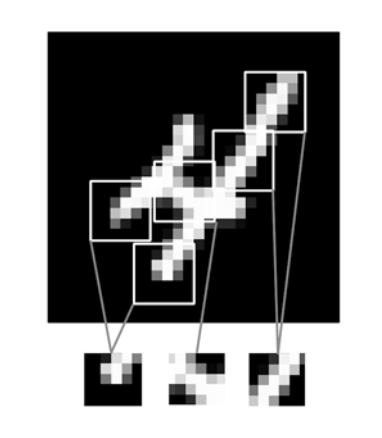
\includegraphics[width=0.7\textwidth]{bilder/convolution_example.PNG}
	\caption{Bilder können in lokale Muster wie Kanten oder Texturen unterteilt werden. Hier wurden drei Muster in dem Bild erkannt\cite{francois}.}
	\label{convolution_example}
\end{figure}

\newpage
~\newline
Grundsätzlich haben CNNs zwei wichtige Eigenschaften\cite{francois}:

\begin{itemize}
	\item \textbf{Translationsinvariante}: Mithilfe dieser Eigenschaft können CNNs nach dem Erlernen eines bestimmten Musters, ortsunabhängig in dem ganzen Bild das Muster wiedererkennen. Bei den klassischen neuronalen Netzen müsste das Muster neu gelernt werden, wenn die Position des Musters aus den Trainingsdaten abweicht. 
	Ein weiterer Vorteil ist, dass weniger Trainingsproben benötigt werden, um Darstellungen zu erlernen, die für die Generalisierung hilfreich sind.
	
	\item \textbf{Räumliche Musterhierarchien}: Da CNNs aus mehreren Faltungsschichten bestehen, lernt die erste Faltungsschicht kleine lokale Muster wie Kanten. Die nächste Schicht lernt größere Muster aus den Merkmalen der ersten beziehungsweise vorherigen Schichten. Dadurch können CNNs immer komplexere und abstraktere visuelle Darstellungen effizient erlernen. Dabei bildet sich eine Hierarchie aus Mustern. Die Abbildung \ref{cat_pattern} zeigt eine solche Hierarchie. Bestehend aus einfachen unterschiedlich aussehenden Kanten werden Konstrukte, zum Beispiel die Nase, Augen und Ohren, gebildet, um eine Katze klassifizieren zu können.
	

	\begin{figure}[h!]
		\centering
		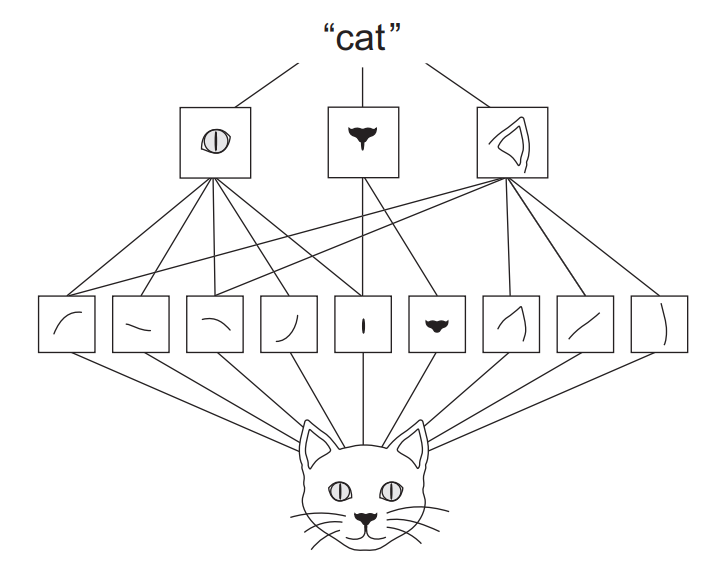
\includegraphics[width=0.7\textwidth]{bilder/cat_pattern.PNG}
		\caption{Lokale Kanten verbinden sich zu lokalen Objekten wie Augen oder Ohren, um die Klasse \glqq Katze\grqq~erkennen zu können\cite{francois}.}
		\label{cat_pattern}
	\end{figure}
	
\end{itemize}



Neben der zwei wichtigsten Eigenschaften arbeiten Faltungsschichten auf einer so genannten Feature-Map mit zwei räumlichen Achsen, hier Höhe und Breite, sowie eine Tiefenachse. Zum Beispiel ist die Dimension der Tiefenachse bei einem RGB-Bild drei, da das Bild drei Farbkanäle beinhaltet, nämlich rot, grün und blau. Die Faltungsoperation extrahiert Felder aus ihrer Input-Feature-Map und wendet die gleiche Transformation auf alle diese Felder an, wodurch eine Output-Feature-Map entsteht. Diese Feature-Map ist immer noch ein 3D-Würfel. Allerdings kann die Tiefe beliebig sein, da die Ausgabetiefe ein Parameter der Ebene ist und die verschiedenen Kanäle in dieser Tiefenachse nicht mehr für bestimmte Farben wie beim RGB-Eingang stehen, sondern für die Anzahl der Filter. Ein Filter kodiert bestimmte Aspekte der Eingangsdaten\cite{francois}. 

Die Funktionsweise einer Faltung lässt sich folgendermaßen erläutern\cite{francois}. Zunächst wird ein Fenster der Größe 3 x 3 oder 5 x 5 über die dreidimensionale Feature-Map verschoben, um ein dreidimensionales Teilstück zu extrahieren. Diese Operation wird an jeder möglichen Stelle ausgeführt. Jedes dreidimensionale Teilstück wird dann in einen eindimensionalen Formvektor transformiert. Alle diese Vektoren werden dann räumlich zu einer dreidimensionalen Feature-Map mit den Dimensionen, also Höhe, Breite und Ausgabetiefe, zusammengefügt. Die Abbildung \ref{feature_map_extraction} visualisiert die beschriebene Schritte.

\begin{figure}[h!]
	\centering
	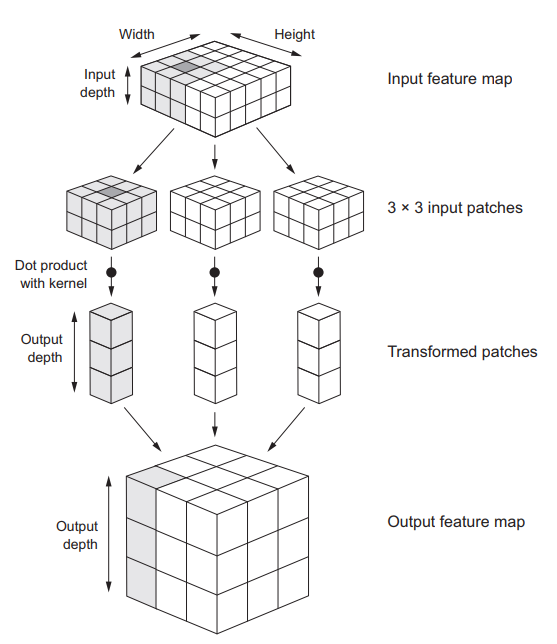
\includegraphics[width=0.7\textwidth]{bilder/feature_map_extraction.PNG}
	\caption{Visualisierung der Zusammensetzung von neuen Feature-Maps mittels der mathematischen Faltung\cite{francois}.}
	\label{feature_map_extraction}
\end{figure}
%% über padding schreiben


\subsection{Poolingschicht}
\label{sec:poolingschicht}
%book i

Die Poolingschicht ist eine Möglichkeit der Nachverarbeitung, wie die Daten in den Feature-Maps nach verarbeitet werden können\cite{francois}. Ein Fenster, das die Größe 2 x 2 hat, durchläuft die Feature-Map und extrahiert Werte. Abhängig von der Operation, zum Beispiel das Maximum, das Minimum oder der Durchschnitt, werden alle umliegenden Werte betrachtet. Ein einzelner Wert repräsentiert die umliegenden Pixel in dem Fensterausschnitt\cite{IntroML}. Ein großer Unterschied zu der Faltungsschicht besteht darin, dass Feature-Maps um den Faktor zwei verkleinert werden, um die Koeffizienten in den Feature-Maps zu reduzieren\cite{francois}. Des Weiteren glättet ein solches Verfahren Feature-Maps. Bei einer Max-Poolingschicht wird ein sehr hoher Wert in die umgebenden Werte einfließen, so dass die genaue Position in der Feature-Map nicht mehr relevant ist. Vielmehr wird nun auf den allgemeinen Bereich, also an und um diese Position herum, fokussiert \cite{IntroML}.


Die Abbildung \ref{cnn_pooling_example} zeigt die Dimensionreduktion nach der Poolingschicht. Das Eingabebild ist zunächst 28 x 28 groß. Nach der mathematischen Faltung in der Faltungsschicht ist die Feature-Map auf 24 x 24 verkleinert. In dieser Feature-Map werden vier benachbarte Werte innerhalb des 2 x 2 großen Fensters anschließend zu einem Wert zusammengeführt, so dass die Größe nun bei 12 x 12 liegt. Außerdem entspricht die Reduzierung der Dimension dem Faktor zwei.


\begin{figure}[h!]
	\centering
	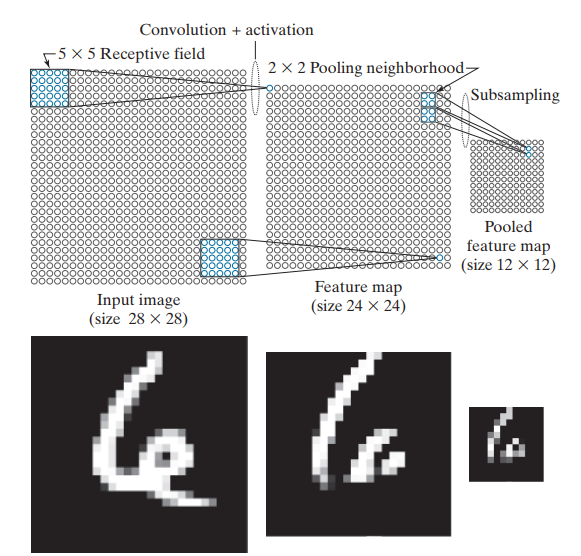
\includegraphics[width=0.75\textwidth]{bilder/convolution_example2.PNG}
	\caption{Veranschaulichung der Konsequenz nach der Poolingschicht. Die Ausgangsgröße der Feature-Map (24 x 24) verkleinert sich auf eine Größe von 12 x 12\cite{Gonzalez2018}.}
	\label{cnn_pooling_example}
\end{figure}



\subsection{Regularisierung}
%TODO: Bessere Abgrenzung von paragraph

%book b 139

Der Begriff Regularisierung beschreibt einen Prozess, welcher die Überanpassung eines Modells reduzieren kann. Es ist eine Möglichkeit, den Lernprozess zu warnen, dass bestimmte Daten ein Rauschen vorweisen oder das Modell auswendig gelernt haben können\cite{Nelli2018}. 


\subsubsection{Gewichtsregulierung}
%book b 139
Falls Daten ein gewisses Rauschen vorweisen, ist es dank der Gewichtsregulierung möglich, die Modellgewichte im Falle einer Überpassung zu bestrafen\cite{Nelli2018,Vasilev2019}. Bei dem Lernverfahren werden die Gewichte der Neuronenverbindungen nach jeder Iteration aktualisiert. Beim Auftreten einer verrauschten Probe kann das Modell fälschlicherweise annehmen, dass diese Probe gültig ist und versucht das Muster, anzupassen\cite{Nelli2018,Subramanian2018}. Durch die Anpassung werden die Gewichte dementsprechend geändert und die Veränderung kann enorm sein. Normalerweise weisen verrauschte Proben keine Ähnlichkeit mit normalen Datenpunkten auf, da sie weit entfernt von ihnen sind. Die Lösung des Problems ist, dass die Gewichte der Kanten zur definierten Verlustfunktion dazu addiert werden und somit ganzheitlich höhere Kosten darstellen. Dann kann das Modell sich selbst abstimmen, um den Verlust zu reduzieren und sorgt dafür, dass die Aktualisierung der Gewichte in die richtige Richtung geht. Die allgemeine Regularisierung lässt sich folgendermaßen beschreiben:

\begin{equation}
Kosten = Verlust + Hyperparameter~x~[Gewichte]
\end{equation}

Dabei entspricht der Hyperparameter dem Ausdruck $\frac{\lambda}{2m}$ und der Wert $\lambda$ wird von dem Anwender definiert. Da einige Regularisierungen existieren, werden hier nur zwei vorgestellt, nämlich L1 und L2.


\paragraph{L1-Regularisierung}
~\newline


Die absoluten Gewichte werden bei der L1-Regularisierung zur Verlustfunktion addiert. Für die Generalisierung des Modells werden die Werte der Gewichte auf null reduziert. Des Weiteren sorgt dieses Verfahren für eine schnellere Berechnung\cite{Nelli2018}.
\newline
Die L1-Regularisierung lässt sich folgendermaßen beschreiben:

\begin{equation}
	Kosten = Verlust + \frac{\lambda}{2m}*\sum\vert\vert Gewichte\vert\vert
\end{equation}



\paragraph{L2-Regularisierung}
~\newline

Bei diesem Verfahren werden die Gewichte quadriert zur Verlustfunktion hinzugefügt. Im Gegensatz zu dem L1-Verfahren werden die Werte der Gewichte auf bei nahezu null reduziert. In den meisten Fällen wird die L2-Regularisierung gegenüber der L1-Regularisierung bevorzugt, um die Überpassung zu reduzieren\cite{Nelli2018}.
\newline
Die mathematische Formulierung kennzeichnet sich durch diese Gleichung:

\begin{equation}
Kosten = Verlust + \frac{\lambda}{2m}*\sum\vert\vert Gewichte\vert\vert^2
\end{equation}

%%erstmal raus
%%\subsubsection{Early-Stopping}
\subsubsection{Dropout-Verfahren}

Für neuronale Netze ist das Dropout-Verfahren eine der effektivsten und am häufigsten verwendeten Regularisierungstechniken. Die Idee hinter diesem Verfahren liegt darin, während des Lernens die Ausgabefunktion in einer Schicht zufällig auf null zu setzen\cite{francois}. Dadurch ändert sich die Struktur des Modells, so dass Variationen an Parametersätzen entstehen\cite{Gonzalez2018}. Des Weiteren gibt die Dropout-Rate an, wie hoch der Anteil der Datenpunkte auf den Wert null gesetzt werden sollen. In der Regel liegt der Anteil zwischen 0.2 und 0.5\cite{francois, Moolayil2018}.

In Abbildung \ref{dropout} werden einige Knoten in dem neuronalen Netz in jeder Schicht nicht mehr angesprochen.

\begin{figure}[h!]
	\centering
	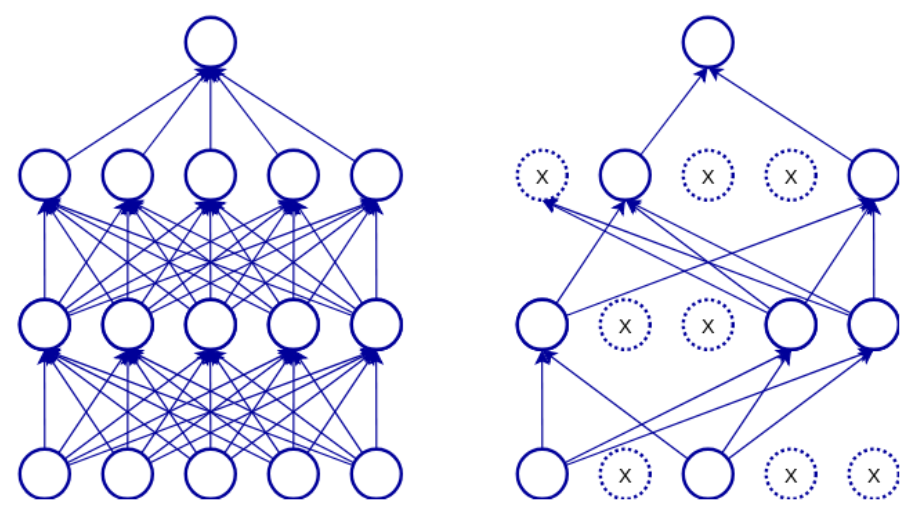
\includegraphics[width=1\textwidth]{bilder/dropout.PNG}
	\caption{In der linken Darstellung wird ein komplett vernetztes Netzwerk angezeigt. Ausgehend von dieser Struktur können einige Knoten in jeder Schicht (rechts) ausgeschlossen werden\cite{Vasilev2019}.}
	\label{dropout}
\end{figure}

\section{Bibliotheken}
%TODO: Tensorflow und GPU Computing/Parallel Computing, book d
%%book h
Zahlreiche Open-Source-Bibliotheken erlauben die Implementierung von tiefen neuronalen Netzen in der Programmiersprache Python. Dabei wird der Code nicht von Grund auf neu geschrieben, weil diese Bibliotheken auf die Grundeinheit für die Datenspeicherung (Tensor) nutzen. Ein Tensor ist eine Verallgemeinerung einer Matrix in höheren Dimensionen bestehend aus mehrdimensionalen Arrays von Basiswerten, die typischerweise von 16 bis 64-Bit Float beziehungsweise Integer repräsentieren. In diesem Abschnitt werden folgende Bibliotheken vorgestellt: Keras und Pytorch\cite{Vasilev2019}.


\subsection{Keras}
%%book i
\label{sec:keras}
Die Bibliothek Keras ermöglicht eine komfortable Definition und Umsetzung von neuronalen Netzen jeglicher Art\cite{francois}. Ursprünglich wurde diese Bibliothek für Forscher entwickelt, um schnelle Experimente zu ermöglichen. Daher verfügt diese Bibliothek über eine integrierte Unterstützung für Faltungsnetzwerke, wiederkehrende Netzwerke (engl. recurrent network) und jede Kombination von beidem. Des Weiteren werden beliebige Netzwerkarchitekturen unterstützt, zum Beispiel Modelle mit mehreren Eingängen
beziehungsweise Ausgängen.

\begin{figure}[h!]
	\centering
	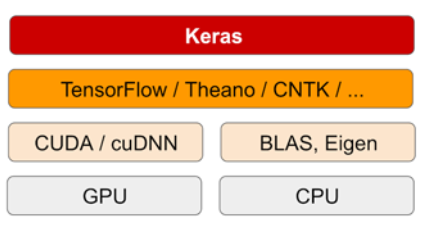
\includegraphics[width=0.7\textwidth]{bilder/keras_backend.PNG}
	\caption{In dieser Grafik wird die Flexibilität von Keras bezüglich des Backends sowie der Prozessoreinheit visualisiert\cite{francois}.}
	\label{keras_backend}
\end{figure}

Da die Bibliothek Keras nicht als Backend fungiert, wird Keras folgende Backends unterstützt: TensorFlow, CNTK und Theano. Jeder Programmiercode, welcher mit Keras geschrieben wurde, kann mit jedem dieser Backends ausgetauscht sowie ausgeführt werden. Hierbei werden keine Anpassungen des Codes benötigt (s. Abbildung \ref{keras_backend})\cite{francois}.  

\subsubsection{Erstellung des Modells}

Die Keras Bibliothek bietet zwei Möglichkeiten, wie ein Modell definiert werden kann. Mit der \textbf{Sequential}-Klasse können linear aufgebaute Modelle, die der häufigsten Netzwerkarchitektur entsprechen, erstellt werden. Mit der \textbf{Functional}-API können beliebige Architekturen gebaut werden, wenn die Struktur der Schichten einem direkten azyklischen Graphen ähnelt. Der Aufbau der zwei Möglichkeiten ist ähnlich. Zunächst müssen Eingabe-Tensoren und Ziel-Tensoren definiert werden. Anschließend wird ein Netzwerk mit Schichten erstellt, welches die Eingaben auf die Ziele abbildet\cite{francois}.

Der Code-Abschnitt \ref{model_seq} zeigt, wie ein Modell mit der \textbf{Sequential}-Klasse erstellt wird. In der ersten Schicht wird die erwartete Form der Eingangsdaten übermittelt.

\begin{lstlisting}[caption={Erstellung eines Modells mit der \textbf{Sequential}-Klasse\cite{francois}.}, label=model_seq]
from keras import models
from keras import layers
model = models.Sequential()
model.add(layers.Dense(32, activation='relu', input_shape=(784,)))
model.add(layers.Dense(10, activation='softmax'))
\end{lstlisting}

Mit der \textbf{Functional}-API werden die Tensoren manipuliert, die vom Modell verarbeitet werden, um diese auf Schichten anzuwenden. Daher werden Tensoren als Funktionsparameter übergeben (s. Code \ref{model_functional}).

\begin{lstlisting}[caption={Ein anderer Ansatz zu der Erstellung eines Modells mittels der \textbf{Functional}-API\cite{francois}.}, label=model_functional]
input_tensor = layers.Input(shape=(784,))
x = layers.Dense(32, activation='relu')(input_tensor)
output_tensor = layers.Dense(10, activation='softmax')(x)
model = models.Model(inputs=input_tensor, outputs=output_tensor)
\end{lstlisting}

\subsubsection{Das Kompilieren eines Modells}
Nach der Erstellung des Modells ist der nächste Schritt die Konfiguration des Trainings\cite{francois}. Diese Konfiguration findet im Kompilierungsschritt statt, in dem die Optimierungs- und Verlustfunktionen angeben werden. Des Weiteren können Metriken benutzt werden, um während des Trainings das Lernen des Modells zu überwachen. Der Code \ref{kcc} zeigt ein Beispiel mit dem RMSprop-Gradientenverfahren sowie der mittleren quadratischen Abweichung als Verlustfunktion. In der Dokumentation von Keras können weitere Optimierungs- und Verlustfunktionen gefunden werden\cite{keras_doc}.


\begin{lstlisting}[caption={Die Kompilierung eines Modells\cite{francois}.}, label=kcc]
from keras import optimizers
model.compile(optimizer=optimizers.RMSprop(lr=0.001),
	loss='mse',
	metrics=['accuracy'])
\end{lstlisting}


\subsubsection{Das Trainieren des Modells}
Um das Training zu starten, werden über die \textit{fit()}-Methode die Eingabedaten und dementsprechend Zieldaten übergeben. Des Weiteren benötigt diese Methode die Anzahl der Epochen sowie die Batchgröße. Als Rückgabe wird ein \textit{History-Objekt} zurückgegeben, welches eine Aufzeichnung der Trainingsverlustwerte und Metrikenwerte in aufeinanderfolgenden Epochen sowie der Validierungsverlustwerte und Validierungsmetrikenwerte enthält\cite{francois}.
Der Code \ref{tkc} zeigt den Aufruf der \textit{fit()}-Methode mit der Batchgröße 128 sowie zehn Epochen. Des Weiteren gibt es weitere Abwandlungen der \textit{fit()}-Methode, die in der Quelle zu finden sind\cite{keras_doc}.


\begin{lstlisting}[caption={Das Starten des Trainings mit der \textit{fit()}-Methode\cite{francois}.}, label=tkc]
model.fit(input_tensor, target_tensor, batch_size=128, epochs=10)
\end{lstlisting}


\subsubsection{Einlesen der Daten}
%%book h
Da Dateien im Bildformat vorliegen können, bietet Keras einen Generator, hier ImageDataGenerator, für das Einlesen an. Mit diesem Generator können die eingelesenen Bilder direkt zufällig manipuliert werden\cite{Vasilev2019}. Der Codeabschnitt \ref{idgc} zeigt wie ein ImageDataGenerator-Objekt mit Breiten- und Höhenverschiebung, horizontalem Spiegeln und einigen Normalisierungen erstellt werden kann. 


\begin{lstlisting}[caption={Vorverarbeitung der Bilder mit der \textbf{ImageDataGenerator}-Klasse\cite{Vasilev2019}.}, label=idgc]
data_generator = ImageDataGenerator(rotation_range=90,
width_shift_range=0.1,
height_shift_range=0.1,
featurewise_center=True,
featurewise_std_normalization=True,
horizontal_flip=True)
data_generator.fit(X_train)
\end{lstlisting}

Weitere Operatoren sind in der Quelle\cite{keras_doc} dokumentiert.

\subsubsection{Callbacks}

Mithilfe von Callbacks kann die Kontrolle während des Trainings sowie das Verständnis, was in dem Modell vor sich geht, erlangt werden. Dadurch können schlechte Ergebnisse vermieden werden, wenn die Callbacks-Funktionen Daten an den Bediener zurücksenden und automatisch Steuerungsentscheidungen auf der Grundlage des aktuellen Zustands treffen. Ein Callback ist ein Objekt, das im Aufruf der \textit{fit()}-Methode an das Modell übergeben wird. Letztendlich wird dieses Objekt von dem Modell an verschiedenen Stellen im Training aufgerufen. Das Callback-Objekt hat Zugriff auf alle verfügbaren Daten über den Zustand des Modells und seine Leistung, so dass es Maßnahmen ergreifen kann. Zwei solcher Maßnahmen werden hier kurz vorgestellt\cite{francois}:

\paragraph{EarlyStopping}
~\newline

Mithilfe des \textit{EarlyStopping}-Callback kann das Training unterbrochen werden, wenn eine zu überwachende Zielgröße für eine bestimmte Anzahl von Epochen keine Verbesserung aufweist. Dadurch kann die Überanpassung des Modells mit steigender Epochenanzahl verhindert werden, wenn das Training rechtzeitig nach der definierten Zielgröße abbricht. Der Code \ref{kces} zeigt die Erstellung eines \textit{EarlyStopping}-Callbacks. Callbacks werden als Parameter in der \textit{fit()}-Methode an das Modell übergeben. Das Modell nimmt eine Liste von Callbacks an. In diesem Beispiel wird die Validierungsgenauigkeit des Modells überwacht. Das Training wird unterbrochen, wenn die Genauigkeit seit mehr als einer Epoche nicht mehr verbessert wird.

\begin{lstlisting}[caption={Das frühe Stoppen des Trainings wird mit dem EarlyStopping-Callback veranlasst\cite{francois}.}, label=kces]
callbacks_list = [
	keras.callbacks.EarlyStopping(
		monitor='acc',
		patience=1,
)]

model.fit(x, y,
	epochs=10,
	batch_size=32,
	callbacks=callbacks_list,
	validation_data=(x_val, y_val))
\end{lstlisting}



\paragraph{ModelCheckpoint}
~\newline

Das \textit{ModelCheckpoint}-Callback wird häufig zusammen mit dem \textit{EarlyStopping}-Callback kombiniert, so dass das Modell während des Trainings kontinuierlich gespeichert werden kann. Des Weiteren besteht die Möglichkeit nur das aktuell beste Modell zu speichern. Der Codeabschnitt \ref{kcmc} veranschaulicht, wie das \textit{ModelCheckpoint}-Callback erstellt wird. Zunächst muss der Pfad des zu speichernden Modells definiert werden. Anschließend wird festgelegt, welche Zielgröße überwacht werden soll. Falls der Parameter \glqq save\_best\_only\grqq~auf wahr gesetzt ist, dann wird das zu speichernde Modell nur überschrieben, wenn sich die Zielgröße verbessert hat. Ansonsten werden die Gewichte des Modells bei jeder Epoche abgespeichert.

\begin{lstlisting}[caption={Mithilfe des ModelCheckpoint-Callbacks wird das beste Modell in dem Training abgespeichert\cite{francois}.}, label=kcmc]
keras.callbacks.ModelCheckpoint(
	filepath='my_model.h5',
	monitor='val_loss',
	save_best_only=True)
\end{lstlisting}



\subsubsection{GPU-Support}
Keras ist in der Lage über TensorFlow oder über andere Backends, den Code sowohl auf CPUs als auch auf GPUs auszuführen. Falls das TensorFlow Backend auf der CPU ausgeführt wird, wird eine Low-Level-Bibliothek für Tensoroperationen namens Eigen verwendet. Falls die Ausführung des Codes über eine Grafikkarte verläuft, dann wird eine Bibliothek verwendet, die für Grafikkarten, zum Beispiel NVIDIA CUDA Deep Neural Network Library (cuDNN), optimiert wurde\cite{francois}. 

\subsection{PyTorch}
\label{sec:pytorch}
Dieser Abschnitt basiert auf dem Buch von Vishnu Subramanian\cite{Subramanian2018}.
 
Für die Erstellung von tiefen Faltungsnetzen kennzeichnet sich PyTorch durch die Benutzerfreundlichkeit und Einfachheit. Viele andere gängige Frameworks, die die Erstellung der Faltungsnetze ermöglichen, verwenden statische Berechnungsgraphen. Die Bibliothek PyTorch verfolgt einen anderen Ansatz und bietet einen dynamischen Berechnungsgraphen an, welcher eine größere Möglichkeit bei der Erstellung von komplexen Architekturen anbietet. Ein weiterer Vorteil von PyTorch ist die Verwendung von Python-Konzepten, zum Beispiel Klassen, Strukturen und bedingte Schleifen, um objektorientiert Faltungsnetze aufbauen zu können. Da PyTorch hauptsächlich für die Forschung entwickelt wurde, wird es in bestimmten Szenarien mit sehr geringen Latenzen nicht für den produktiven Einsatz empfohlen.

\subsubsection{Erstellung des Modells}

Alle neuronale Netze werden in PyTorch als Klassen definiert. Des Weiteren wird diese Klasse von \textbf{nn.Module} vererbt. Grundsätzlich sollte ein Konstruktor erstellt werden, um die Initialisierung der Schichten für das Netzwerk zu realisieren. In der PyTorch Dokumentation sind verschiedene Arten von Schichten aufgelistet\cite{pytorch_doc}. In der \textit{forward()}-Methode werden die Eingabedaten an die Schichten übergeben, die im Konstruktor initialisiert wurden. Anschließend wird die Ausgabe zurückgegeben.

Der folgende Codeausschnitt \ref{pytorch_erstellung} zeigt, wie ein tiefes, neuronales Netz in PyTorch implementiert werden kann.

\begin{lstlisting}[caption={Veranschaulichung der typischen Klassenstruktur eines neuronalen Netzes\cite{Subramanian2018}.}, label=pytorch_erstellung]
class MyFirstNetwork(nn.Module):
	def __init__(self, input_size, hidden_size, output_size):
		super(MyFirstNetwork, self).__init__()
		self.layer1 = nn.Linear(input_size, hidden_size)
		self.layer2 = nn.Linear(hidden_size, output_size)
		
	def __forward__(self, input):
		out = self.layer1(input)
		out = nn.ReLU(out)
		out = self.layer2(out)
		return out
\end{lstlisting}

\subsubsection{Das Trainieren des Modells}

Um das Training zu starten, müssen zunächst die Hyperparameter definiert werden. In dem Code \ref{tpt} wird die Lernrate auf 0.001 gesetzt. Die Verlustfunktion ist in diesem Modell die Kreuzentropie und das Lernverfahren wird mit dem stochastischen Gradientenverfahren (engl. SGD) durchgeführt. Die \textit{StepLR()}-Funktion passt die Lernrate während des Trainings dynamisch an.  

\begin{lstlisting}[caption={Definition der Hyperparameter, die in der Training-Methode benötigt werden\cite{Subramanian2018}.}, label=tpt]
learning_rate = 0.001
criterion = nn.CrossEntropyLoss()
optimizer_ft = optim.SGD(model_ft.parameter(),lr=0.001, momentum=0.9)
exp_lr_scheduler.StepLR(optimizer_ft, step_size=7,gamma=0.1)
\end{lstlisting}

Die Methode \textit{$train\_Model$} in dem Code \ref{headh_train} nimmt ein Modell mit den Hyperparametern an und wird für 25 Epochen trainiert. Die Methode selbst lässt sich in vier Abschnitten einteilen. Zunächst erhält das Modell die Bilddateien und berechnet daraus den Verlust.

\begin{lstlisting}[caption={Berechnung der Verluste in der Training-Methode\cite{Subramanian2018}.}, label=headh_train]
def train_model(model, criterion, optimizer, scheduler, num_epochs=25):
	best_model_wts = model.state_dict()
	best_acc = 0.0
	
	for epoch in range(num_epochs):
		for phase in ['train', 'valid']:
			if phase == 'train':
				scheduler.step()
				model.train(True)
			else:
				model.train(False)
				
			running_loss = 0.0
			running_corrects = 0
			
			for data in dataloaders[phase]:
				inputs, labels = data
				inputs, labels = Variable(inputs), Variable(labels)
				
				#zero the parameter gradients
				optimizer.zero_grad()
				
				#forward
				outputs = model(inputs)
				_, preds = torch.max(outputs.data, 1)
				loss = criterion(outputs, labels)
\end{lstlisting}
Während der Trainingsphase wird der Verlust rückwärts propagiert. In der Validierungs- und Testphase werden die Gewichte nicht aktualisert (s. Code \ref{bwppt}).

\begin{lstlisting}[caption={Aktualisierung der Gewichte in der Training-Methode\cite{Subramanian2018}.}, label=bwppt]		
				#backwards
				if phase == 'train':
					loss.backward()
					optimizer.step()
\end{lstlisting}
Im Codeabschnitt \ref{cumulation} wird der Verlust in Batches für jede Epoche kumuliert.

\begin{lstlisting}[caption={Berechnung der Verluste in Batches in der Training-Methode\cite{Subramanian2018}.}, label=cumulation]					
				#statistics
				running_loss += loss.data[0]
				running_corrects += torch.sum(preds == labels.data)
			
			epoch_loss = running_loss / dataset_sizes[phase]
			epoch_acc = running_corrects / dataset_sizes[phase]
			
\end{lstlisting}
			
Der letzte Schritt ist nun das Speichern der Gewichte von dem besten Modell (s. Code \ref{pytorch_save}).
\begin{lstlisting}[caption={Festlegung des besten Modells in der Training-Methode\cite{Subramanian2018}.}, label=pytorch_save]						
			#copy the model
			if phase == 'valid' and epoch_acc > best_acc:
				best_acc = epoch_acc
				best_model_wts = model.state_dict()
	
	#load best model weights
	model.load_state_dict(best_model_wts)
	return model
\end{lstlisting}

\subsubsection{Einlesen der Daten}

Das \textbf{torchvision.datasets}-Paket wird von PyTorch bereitgestellt und wird mittels der Klasse \textbf{ImageFolder} verwendet, um das Laden von Bildern mit den dazugehörigen Labels zu ermöglichen. Nach erfolgreichem Laden der Bilder können Vorverarbeitungsschritte ausgeführt werden. Zum Beispiel können alle Bilder auf eine Größe skaliert werden. Typischerweise wird der Datensatz mit dem Mittelwert und der Standardabweichung des Datensatzes normalisiert. Nach den Vorverarbeitungsschritten können die Daten zu einem PyTorch-Tensor konvertiert werden. 

\begin{lstlisting}[caption={Das Einlesen der Bilddateien wird mit der Klasse \textit{ImageFolder} realisiert\cite{Subramanian2018}.}, label=eddpt]
simple_transform=transforms.compose([transforms.Scale((244,244)),
							transforms.ToTensor(),
							transforms.Normalize([0.485, 0.456, 0.406],
												[0.229, 0.224, 0.225])])
train = ImageFolder('dogsandcats/train/', simple_transform)
valid = ImageFolder('dogsandcats/valid/', simple_transform)
\end{lstlisting}

Der Codeabschnitt \ref{eddpt} zeigt, wie die Bilder mit der Klasse ImageFolder geladen und anschließend diese mit einer einfachen Transformation verändert werden. Hierbei werden die Bilder auf die Größe 244 x 244 skaliert. Anschließend werden die Bilddateien als Tensor konvertiert und mit dem Mittelwert und der Standardabweichung normalisiert. Nach der Erstellung des Objekts für die Transformation wird dieses Objekt als Parameter an die \textbf{ImageFolder}-Klasse übergeben.

\subsubsection{GPU-Support}

Vortrainierte Modelle können auf der Grafikkarte ausgeführt werden. Hierfür muss das Modell die Methode \textit{cuda()} aufgerufen werden. Der Code \ref{gpupt} zeigt diesen Aufruf. 

\begin{lstlisting}[caption={Mit der \textit{cuda()}-Methode wird das Modell auf der Grafikkarte trainiert\cite{Subramanian2018}.}, label=gpupt]
if is_cuda:
	model = model.cuda()
\end{lstlisting}

Für selbst erstellte Modelle muss zunächst das Objekt erlangt werden, welches den Zugriff auf die Grafikkarte hat. Anschließend werden das neuronale Netz und die Daten, also Datenpunkte sowie die Labels, auf die Grafikkarte transferiert (s. Code \ref{transformiert}). 


\begin{lstlisting}[caption={Die Daten und das Modell werden auf die Grafikkarte übertragen, um dort ausgeführt werden zu können\cite{Subramanian2018}.}, label=transformiert]
device = torch.device("cuda:0" if torch.cuda.is_available())

net.to(device)

inputs, labels = data[0].to(device), data[1].to(device)
\end{lstlisting} 

